\documentclass[10pt]{article}
\usepackage[polish]{babel}
\usepackage[utf8]{inputenc}
\usepackage[T1]{fontenc}
\usepackage{amsmath}
\usepackage{amsfonts}
\usepackage{amssymb}
\usepackage[version=4]{mhchem}
\usepackage{stmaryrd}
\usepackage{graphicx}
\usepackage[export]{adjustbox}
\graphicspath{ {./images/} }
\usepackage{bbold}

\title{XXXVII \\
 KORESPONDENCYJNY KURS Z MATEMATYKI }

\author{}
\date{}


\begin{document}
\maketitle
\section*{PRACA KONTROLNA nr 1 - POZIOM PODSTAWOWY}
październik 2007r.

\begin{enumerate}
  \item Pan Kowalski wpłacił pewną sumę na lokatę oprocentowaną w wysokości $8 \%$ w skali roku, przy czym odsetki naliczane są kwartalnie. W ciągu rozważanego roku inflacja wyniosła 4\%. Jakie jest realne roczne oprocentowanie lokaty Pana Kowalskiego, tzn. o ile procent więcej warte są pieniądze, które Pan Kowalski miał na koncie po roku od tych, które wpłacił? Wynik podać z dokładnością do setnych części procenta.
  \item Liczba $p=\frac{(\sqrt[3]{54}-2)(9 \sqrt[3]{4}+6 \sqrt[3]{2}+4)-(2-\sqrt{3})^{3}}{\sqrt{3}+(1+\sqrt{3})^{2}}$ jest miejscem zerowym funkcji $f(x)=a x^{2}+b x+c$. Wyznaczyć współczynniki $a, b, c$ oraz drugie miejsce zerowe tej funkcji wiedząc, że największą wartością funkcji jest 4, a jej wykres jest symetryczny względem prostej $x=1$.
  \item Dwie styczne do okręgu o promieniu 6 przecinają się pod kątem $60^{\circ}$. Obliczyć pole obszaru ograniczonego odcinkami tych stycznych i krótszym z łuków, na jakie okrąg podzielony jest punktami styczności. Wyznaczyć promień okręgu wpisanego w ten obszar.
  \item Niech
\end{enumerate}

$$
f(x)=\left\{\begin{array}{lll}
\frac{1}{x-1}, & \text { gdy } & |x-1| \geqslant 1 \\
x^{2}-x-1, & \text { gdy } & |x-1|<1
\end{array}\right.
$$

a) Obliczyć $f\left(-\frac{2}{3}\right), f\left(\frac{1+\sqrt{3}}{2}\right)$ oraz $f(\pi-1)$.\\
b) Narysować wykres funkcji $f$ i na jego podstawie podać zbiór wartości funkcji.\\
c) Rozwiązać nierówność $f(x) \geqslant-\frac{1}{2}$ i zaznaczyć na osi $0 x$ zbiór jej rozwiązań.\\
5. Pole przekroju graniastosłupa prawidłowego o podstawie kwadratowej płaszczyzną przechodzącą przez przekątną graniastosłupa i środki przeciwległych krawędzi bocznych jest 3 razy większe niż pole podstawy. Wyznaczyć tangens kąta nachylenia przekątnej graniastosłupa do podstawy. Obliczyć pole powierzchni całkowitej tego graniastosłupa wiedząc, że pole rozważanego przekroju równe jest 10 .\\
6. Jeden z wierzchołków trójkąta prostokątnego o polu 7,5 jest punktem przecięcia prostych $k: x-y+3=0$ oraz $l: 2 x+y=0$. Wyznaczyć pozostałe wierzchołki wiedząc, że leżą one na prostych $k$ i $l$, a wierzchołek kąta prostego jest na prostej $l$. Sporządzić staranny rysunek.

\section*{PRACA KONTROLNA nr 1 - POZIOM ROZSZERZONY}
\begin{enumerate}
  \item Narysować wykres funkcji $f(x)=\left\{\begin{array}{lll}\left|3^{x}-1\right| & \text { dla } & x \leqslant 1 \\ \frac{3-x}{x} & \text { dla } & x>1\end{array}\right.$. Posługując się nim podać wzór i narysować wykres funkcji $g(m)$ określającej liczbę rozwiązań równania $f(x)=m$, gdzie $m$ jest parametrem rzeczywistym.
  \item Rozwiązać równanie $\frac{\sin 3 x}{\cos x}=\operatorname{ctg} x-\operatorname{tg} x$.
  \item Napisać równanie stycznej $k$ do wykresu funkcji $f(x)=x^{2}-4 x+3$ w punkcie $\left(x_{1}, 0\right)$, gdzie $x_{1}$ jest najmniejszym miejscem zerowym tej funkcji. Znaleźć punkt przecięcia tej stycznej ze styczną do niej prostopadłą . Sporządzić staranny rysunek.
  \item Rozwiązać nierówność $\log _{2}(x-1)-\log _{\frac{1}{2}}(4-x)-\log _{\sqrt{2}}(x-2) \leqslant 0$.
  \item Rozwiązać nierówność $\sqrt{x^{2}-1}+1+\frac{1}{\sqrt{x^{2}-1}}+\ldots \geqslant \frac{9}{2}$, gdzie lewa strona jest sumą wyrazów nieskończonego ciągu geometrycznego.
  \item W stożek wpisano kulę, a następnie w obszar zawarty między tą kulą i wierzchołkiem stożka wpisano kulę o objętości 8 razy mniejszej. Obliczyć stosunek objętości stożka do objętości kuli na nim opisanej.
  \item Trzy liczby dodatnie tworzą ciąg geometryczny. Suma tych liczb równa jest 26, a suma ich odwrotności wynosi $0.7(2)$. Wyznaczyć te liczby.
  \item Pole powierzchni bocznej ostrosłupa prawidłowego czworokątnego jest 2 razy większe niż pole podstawy. W trójkąt otrzymany w przekroju ostrosłupa płaszczyzną przechodzącą przez jego wysokość i przekątną podstawy wpisano kwadrat, którego jeden bok jest zawarty w przekątnej podstawy. Obliczyć stosunek pola tego kwadratu do pola podstawy ostrosłupa. Sporządzić staranny rysunek.
  \item Wykonać działania i zapisać w najprostszej postaci wyrażenie
\end{enumerate}

$$
s(a, b)=\left(\frac{a^{2}+b^{2}}{a^{2}-b^{2}}-\frac{a^{3}+b^{3}}{a^{3}-b^{3}}\right):\left(\frac{a^{2}}{a^{3}-b^{3}}-\frac{a}{a^{2}+a b+b^{2}}\right) .
$$

Wyznaczyć wysokość trójkąta prostokątnego wpisanego w okrąg o promieniu 6 opuszczoną z wierzchołka kąta prostego wiedząc, że tangens jednego z kątów ostrych tego trójkąta równy jest $s(\sqrt{5}+\sqrt{3}, \sqrt{5}-\sqrt{3})$.\\
4. Wielomian $W(x)=x^{3}-x^{2}+b x+c$ jest podzielny przez $(x+3)$, a reszta z dzielenia tego wielomianu przez $(x-3)$ równa jest 6 . Wyznaczyć $b$ i $c$, a następnie rozwiązać nierówność $(x+1) W(x-1)-(x+2) W(x-2) \leqslant 0$.\\
5. W ramach przygotowań do EURO 2012 zaplanowano budowę kompleksu sportowego złożonego z czterech jednakowych hal sportowych w kształcie półkul o środkach w rogach kwadratu o boku 100 m i piątej hali w kształcie półkuli stycznej do czterech pozostałych. Jakie powinny być wymiary tych hal, by koszt ich budowy był najmniejszy, jeżeli wiadomo, że jest on proporcjonalny do pola powierzchni dachu hali?\\
6. W trójkącie prostokątnym o kącie prostym przy wierzchoku $C$ na przedłużeniu przeciwprostokątnej $A B$ odmierzono odcinek $B D$ tak, że $|B D|=|B C|$. Wyznaczyć $|C D|$ oraz obliczyć pole trójkta $\triangle A C D$, jeżeli $|B C|=5,|A C|=12$. Sporządzić staranny rysunek.

\section*{PRACA KONTROLNA nr 2 - POZIOM ROZSZERZONY}
\begin{enumerate}
  \item Znaleźć wszystkie wartości parametru rzeczywistego $m$, dla których pierwiastki trójmianu kwadratowego $f(x)=(m-2) x^{2}-(m+1) x-m$ spełniają nierówność $\left|x_{1}\right|+\left|x_{2}\right| \leqslant 1$.
  \item Wyznaczyć dziedzinę funkcji $f(x)=\frac{\sqrt{2^{4-x^{2}}-4^{x}}}{\log \left(2-x-x^{2}-\ldots\right)}$.
  \item Grupa 175 robotników miała wykonać pewną pracę w określonym terminie. Po upływie 30 dni wspólnej pracy przesyłano codziennie po 3 robotników na inne stanowiska, wskutek czego robota została wykonana z opóźnieniem 21 dni. W ciągu ilu dni miała być wykonana praca według planu?
  \item Wyznaczyć promień okręgu opisanego na czworokącie $A B C D$, w którym kąt przy wierzchołku $A$ ma miarę $\alpha$, kąty przy wierzchołkach $B, D$ są proste oraz $|B C|=a,|A D|=b$. Sporządzić staranny rysunek.
  \item Narysować staranny wykres funkcji $f(x)=\frac{\sin 2 x-|\sin x|}{\sin x}$. W przedziale $[0, \pi]$ wyznaczyć rozwiązania nierówności $f(x)<2(\sqrt{2}-1) \cos ^{2} x$.
  \item Pole przekroju graniastosłupa prawidłowego o podstawie kwadratowej płaszczyzną przechodzącą przez przekątną graniastosłupa i środek jednej z krawędzi podstawy jest 3 razy większe niż pole podstawy. Wyznaczyć tangens kąta nachylenia przekątnej graniastosłupa do podstawy. Obliczyć pole powierzchni całkowitej tego graniastosłupa wiedząc, że pole rozważanego przekroju równe jest 15 . Sporządzić staranny rysunek.
\end{enumerate}

\section*{PRACA KONTROLNA nr 3 - POZIOM PODSTAWOWY}
grudzień 2007r.

\begin{enumerate}
  \item Rozwiązać równanie
\end{enumerate}

$$
\sqrt{3-x}+\sqrt{3 x-2}=2
$$

\begin{enumerate}
  \setcounter{enumi}{1}
  \item Sześć kostek sześciennych o objętościach $1,2,4,8,16$ i $32 \mathrm{dm}^{3}$ ustawiono w piramidę, układając jedną kostkę na drugiej poczynając od największej. Czy wysokość piramidy przekroczy 120 cm ? Odpowiedź uzasadnić bez prowadzenia obliczeń przybliżonych.
  \item ${ }^{1}$ )Pan W wybrał się na spacer do parku mającego kształt prostokąta o wymiarach 400 m na 300 m , podzielonego alejkami na 12 kwadratów o boku 100 m , jak na rysunku poniżej. Postanowił przejść od punktu $A$ do $B$, łącznie 700 m , wybierając przypadkowo alejkę na każdym rozwidleniu. Jakie jest prawdopodobieństwo, że Pan W przejdzie środkową alejką oznaczoną na rysunku $x$ ?\\
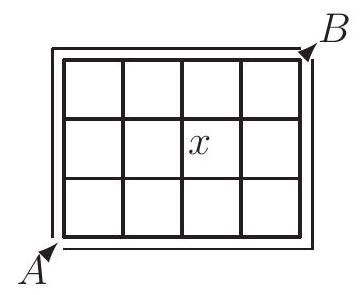
\includegraphics[max width=\textwidth, center]{2024_11_16_dea50acf0e4fa63c62acg-05}
  \item Podstawą trójkąta równoramiennego jest odcinek $A B$ o końcach $A(-1,1), B(3,3)$, a wierzchołek $C$ leży na paraboli o równaniu $y^{2}=x+1$. Wyznaczyć współrzędne wierzchołka $C$ oraz pole trójkąta $A B C$. Sporządzić rysunek.
  \item Na jednym rysunku sporządzić dokładne wykresy funkcji $\sin x, \cos x, \operatorname{tg} x$ oraz $\operatorname{ctg} x$ w przedziale $\left(0, \frac{\pi}{2}\right)$ i zaznaczyć na nich
\end{enumerate}

$$
\operatorname{ctg}\left(\cos \frac{\pi}{4}\right), \cos \left(\sin \frac{\pi}{3}\right), \sin \left(\cos \frac{\pi}{3}\right), \operatorname{tg}\left(\sin \frac{\pi}{2}\right) .
$$

Uporządkować powyższe liczby od najmniejszej do największej. Uzasadnić te relacje za pomocą odpowiednich nierówności.\\
6. W ostrosłupie prawidłowym trójkątnym kąt między ścianami bocznymi ma miarę $\alpha$, a odległość krawędzi podstawy od przeciwległej krawędzi bocznej jest równa $d$. Obliczyć objętość ostrosłupa.

\section*{PRACA KONTROLNA nr 3 -POZIOM ROZSZERZONY}
\begin{enumerate}
  \item Stosując zasadę indukcji matematycznej, udowodnić prawdziwość wzoru
\end{enumerate}

$$
\binom{3}{2}+\binom{5}{2}+\ldots+\binom{2 n+1}{2}=\frac{n(n+1)(4 n+5)}{6} \quad \text { dla } n \geqslant 1
$$

\begin{enumerate}
  \setcounter{enumi}{1}
  \item Wojtuś wylosował jedną monetę ze skarbonki zawierającej 3 złotówki, 4 dwuzłotówki i 3 pięciozłotówki. Następnie, w zależności od wyniku pierwszego losowania, wylosował jeszcze trzy monety, gdy za pierwszym razem otrzymał złotówke, dwie monety, gdy pierwsza była dwuzłotówką oraz jedną monetę, gdy w pierwszym losowaniu dostał pięciozłotówkę. Obliczyć prawdopodobieństwo, że, postępując w ten sposób, zgromadził łącznie co najmniej 8 złotych.
  \item Jednym z wierzchołków kwadratu jest punkt $A(2,2)$, a środkiem jednego z przeciwległych boków jest punkt $M\left(-\frac{1}{2},-\frac{1}{2}\right)$. Wyznaczyć współrzędne pozostałych wierzchołków oraz równanie okręgu opisanego na tym kwadracie.
  \item Rozwiązać nierówność
\end{enumerate}

$$
\frac{1}{\sqrt{3^{x+1}-2}} \geqslant \frac{1}{4-(\sqrt{3})^{x+2}} .
$$

\begin{enumerate}
  \setcounter{enumi}{4}
  \item W ostrosłup prawidłowy trójkątny wpisano walec, którego podstawa leży na podstawie ostrosłupa. Średnica podstawy walca jest równa jego wysokości. Znaleźć tangens kąta nachylenia krawędzi bocznej ostrosłupa do podstawy, dla którego stosunek objętości walca do objętości ostrosłupa jest największy. Podać ten największy stosunek w procentach.
  \item Długości boków trapezu opisanego na okręgu o promieniu $R$ tworzą ciąg arytmetyczny, przy czym najkrótszy bok ma długość $\frac{3}{4} R$. Obliczyć długości obu podstaw trapezu oraz cosinus kąta pomiędzy przekątnymi. Sporządzić rysunek przyjmując $R=2 \mathrm{~cm}$.
\end{enumerate}

\section*{PRACA KONTROLNA nr 4 - POZIOM PODSTAWOWY}
styczeń 2008r.

\begin{enumerate}
  \item Ramka z drutu o długości $l$ ma kształt kwadratu zakończonego trójkątem równoramiennym, jak na rysunku. Bok kwadratu wynosi $a$, natomiast ramię trójkąta równe jest $b$. Wyznaczyć $a$ i $b$ tak, by pola kwadratu i trójkąta były jednakowe.\\
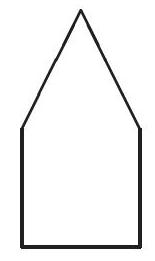
\includegraphics[max width=\textwidth, center]{2024_11_16_dea50acf0e4fa63c62acg-07}
  \item Niech
\end{enumerate}

$$
\begin{aligned}
& A=\{(x, y): x \in \mathbb{R}, y \in \mathbb{R}, y=-x+a, a \in\langle-2,2\rangle\} \\
& B=\left\{(x, y): x \in \mathbb{R}, y \in \mathbb{R}, y=k x, k \in\left\langle\frac{1}{2}, 1\right\rangle\right\} .
\end{aligned}
$$

W prostokątnym układzie współrzędnych narysować zbiór $A \cap B$ i obliczyć jego pole. Sprawdzić, czy punkt $\left(\frac{1}{2}, \frac{3}{4}\right)$ należy do zbioru $A \cap B$.\\
3. Dany jest stożek ścięty, w którym pole dolnej podstawy jest 4 razy większe od pola górnej. W stożek wpisano walec tak, że dolna podstawa walca leży na dolnej podstawie stożka, a brzeg górnej podstawy leży na jego powierzchni bocznej. Jaką część objętości stożka ściętego stanowi objętość walca, jeżeli wysokość walca jest 3 razy mniejsza od wysokości stożka? Odpowiedź podać w procentach z dokładnością do jednego promila. Sporządzić staranny rysunek przekroju osiowego bryły.\\
4. Rozwiązać nierówność $f(x)+3 x>1$, gdzie $f(x)=\frac{1-3 x}{\sqrt{2-\frac{3 x+1}{x-2}}}$.\\
5. Dane są dwa ciągi $a_{n}=\frac{1}{n}$ oraz $b_{n}=\frac{n-2}{(n+2)(n+4)}$. Zbadać monotoniczność ciągu

$$
c_{n}=(n-1) a_{n+1}+2 b_{2 n}
$$

Czy ciąg $c_{n}$ jest ograniczony? Dla jakich $n$ spełniona jest nierówność $\frac{3}{4}<c_{n}<1$ ?\\
6. Okręgi o promieniach $r$ i $2 r$ przecinają się w punktach $A$ i $B$, będących wierzchołkami trójkąta równobocznego $A B C$ wpisanego w jeden z okręgów. Obliczyć pole deltoidu $A D B C$, którego wierzchołek $D$ leży na drugim okręgu oraz wyznaczyć sinus kąta przy wierzchołku $D$.

\section*{PRACA KONTROLNA nr 4 - POZIOM ROZSZERZONY}
\begin{enumerate}
  \item Dany jest romb $A B C D$ o boku $a$ i kącie ostrym $\alpha$. Z wierzchołka $A$ kąta ostrego poprowadzono dwa jednakowej długości odcinki o końcach zawartych w bokach $B C$ i $C D$. Wyznaczyć długości tych odcinków oraz sinusy kątów, na jaki został podzielony kąt $\alpha$ wiedząc, że pole środkowego deltoidu jest równe połowie pola danego rombu.
  \item Napisać równanie stycznej do krzywej $f(x)=\frac{x}{x^{2}-1}$ w punkcie $x_{0}=2$. Wykazać, że obrazem tej stycznej w symetrii względem punktu $(0,0)$ jest prosta, która jest styczną do tej samej krzywej. Wyznaczyć odległość między tymi stycznymi.
  \item Niech
\end{enumerate}

$$
\begin{aligned}
& A=\{(x, y): x \in \mathbb{R}, y \in \mathbb{R},|x-1|+x \geqslant y+|y-2|\} \\
& B=\left\{(x, y): x \in \mathbb{R}, y \in \mathbb{R},|x-1|+\frac{1}{4}|y| \leqslant 1\right\}
\end{aligned}
$$

Na płaszczyźnie $O X Y$ narysować zbiory $A \cap B$ oraz $B^{\prime} \backslash A$.\\
4. Dane jest równanie

$$
8(\sin \alpha+4) x^{2}-8(\sin \alpha+1) x+1=0
$$

gdzie $\alpha \in\langle 0,2 \pi\rangle$. Dla jakich wartości kąta $\alpha$ suma odwrotności pierwiastków tego równania jest równa co najmniej $8\left(\cos \alpha-(\cos \alpha)^{-1}+1\right)$ ?\\
5. Zbadać funkcję $f(m)=\frac{y}{x}$, gdzie para $x$ i $y$ jest rozwiązaniem układu równań

$$
\left\{\begin{aligned}
(m-2) x+(m+2) y & =m^{2}-1 \\
(m+2) x+(m-2) y & =m^{2}+1
\end{aligned}\right.
$$

z parametrem rzeczywistym $m$. Sporządzić wykres funkcji $f(m)$.\\
6. W stożek o promieniu podstawy $r$ i tworzącej $l$ wpisano ostrosłup prawidłowy trójkątny tak, że wierzchołek tego ostrosłupa pokrywa się ze środkiem podstawy stożka, a pozostałe wierzchołki leżą na ścianie bocznej stożka. Jaka jest maksymalna objętość tego ostrosłupa? Sporządzić staranny rysunek.

\begin{enumerate}
  \item Ile razy objętość ostrosłupa trójkątnego prawidłowego opisanego na stożku o objętości $V$ jest większa od objętości ostrosłupa trójkątnego prawidłowego wpisanego w ten stożek?
  \item Rozwiązać nierówność
\end{enumerate}

$$
\left|4 x^{2}-4\right|+2 x \geqslant|1-x|+2
$$

\begin{enumerate}
  \setcounter{enumi}{2}
  \item Kamilek ma 2 latka i 85 cm wzrostu. Przez kolejne 3 lata będzie rósł średnio 1 cm miesięcznie. Potem w ciągu każdych 10 miesięcy będzie rósł o $10 \%$ wolniej niż w poprzednim okresie. Jaki wzrost będzie miał chłopczyk w dniu swoich 15 -tych urodzin? Wynik podać z dokładnością do 5 mm .
  \item Uzasadnić, wykonując odpowiednie obliczenia, że z kartki papieru w kształcie sześciokąta foremnego o boku $a=2(1+\sqrt{3})$ można wyciąć 19 kółek o promieniu 1. Czy istnieje mniejszy sześciokąt foremny, z którego można wyciąć taką samą ilość identycznych kółek?
  \item Punkty $(1,1)$ i $(5,4)$ są dwoma wierzchołkami rombu o polu 15. Opisać konstrukcje wszystkich rombów spełniających podane warunki. Wyznaczyć współrzędne pozostałych wierzchołków, przy założeniu, że nie wszystkie wierzchołki leżą w I ćwiartce układu współrzędnych.
  \item Wyznaczyć równanie krzywej będącej zbiorem wszystkich środków cięciw paraboli $y=(x-1)^{2}+1$ przechodzących przez punkt $P(-1,2)$.\\
(Wsk. Zauważyć, że jeżeli $x_{1}, x_{2}$ są pierwiastkami trójmianu kwadratowego $y=a x^{2}+b x+c$, to prawdziwa jest równość $x_{1}+x_{2}=\frac{-b}{a}$.)
\end{enumerate}

\section*{PRACA KONTROLNA nr 5 - POZIOM ROZSZERZONY}
\begin{enumerate}
  \item Rozwiązać równanie
\end{enumerate}

$$
\operatorname{tg}^{2} x+\operatorname{tg}^{4} x+\cdots=\frac{1}{2}
$$

w którym lewa strona jest sumą wyrazów nieskończonego ciągu geometrycznego.\\
2. Pani Józefa wpłaciła do banku pewien kapitał $K_{0}$ na okres jednego roku na lokatę oprocentowaną $P \%$ w skali roku, przy czym kapitalizacja odsetek następuje $N$ razy rocznie. Uzasadnić indukcyjnie, że wzór $K_{n}=K_{0}\left(1+\frac{P}{100 N}\right)^{n}$ okeśla stan konta pani Józefy po $n$-tym okresie kapitalizacyjnym. Sprawdzić, jaki będzie stan konta pani Józefy po roku przy założeniu, że wpłaci ona $10.000,00 \mathrm{zł}$ na $6 \%$, a odsetki kapitalizowane będą co miesiąc.\\
3. Zaznaczyć na płaszczyźnie zbiór rozwiązań nierówności

$$
\log _{\frac{1}{2}}\left(3 \log _{x}(2 y)\right) \geqslant 0
$$

\begin{enumerate}
  \setcounter{enumi}{3}
  \item W koło o promieniu $R$ wpisano trójkąt, którego pole stanowi czwartą część pola koła, a jeden z kątów ma miarę $\alpha$. Obliczyć iloczyn oraz sumę kwadratów długości boków tego trójkąta.
  \item Wyznaczyć równanie krzywej będącej zbiorem wszystkich środków okręgów stycznych do prostej $y=2$ i przechodzących przez początek układu współrzędnych. Spośród rozważanych okręgów narysować wszystkie okręgi styczne do jednej z osi układu współrzędnych i wyznaczyć równanie okręgu przechodzącego przez ich środki.
  \item Na dnie naczynia w kształcie walca umieszczono 6 małych kulek o promieniu $R$ w taki sposób, że każda z nich jest styczna do dwu innych kulek i ściany bocznej naczynia. Następnie umieszczono w nim kulę o promieniu $2 R$ styczną do każdej z małych kulek oraz górnej podstawy walca. Sprawdzić, ile wody zmieści się w tak zapełnionym naczyniu.
\end{enumerate}

\section*{PRACA KONTROLNA nr 6 - POZIOM PODSTAWOWY}
marzec 2008r.

\begin{enumerate}
  \item Dwa naczynia zawierają w sumie 40 litrów wody. Po przelaniu pewnej części wody pierwszego naczynia do drugiego, w pierwszym naczyniu zostało trzy razy mniej wody niż w drugim. Gdy następnie przelano taką samą część wody drugiego naczynia do pierwszego, okazało się, że w obu naczyniach jest tyle samo płynu. Obliczyć, ile wody było pierwotnie w każdym naczyniu i jaką jej część przelewano.
  \item Obwód trójkąta równoramiennego równy jest 20. Jakie powinny być jego boki, by objętość bryły otrzymanej przez obrót tego trójkąta wokół podstawy była największa?
  \item Student opracował 28 spośród 45 przygotowanych na egzamin tematów. Losuje trzy tematy. Jeżeli odpowie poprawnie na wszystkie, to dostanie ocenę bardzo dobrą, jeżeli na dwa - dobrą, a jeżeli na jedno - dostateczną. Jakie jest prawdopodobieństwo, że:\\
a) dostanie przynajmniej db? b) zda egzamin?
  \item Narysować staranny wykres funkcji $f(x)=x^{2}-2|x|-3$, wyznaczyć jej miejsca zerowe i zbiór wartości. Wykorzystując wykres funkcji $f$ :\\
a) narysować wykres funkcji $h(x)=x^{2}-2 x-2|x-1|-1$.\\
b) posługując się powyższymi wykresami określić, dla jakich wartości parametru rzeczywistego $m$ równanie $f(x)=h(x)+m$ ma dokładnie jedno rozwiązanie.
  \item Państwo Kowalscy są właścicielami działki budowlanej w kształcie trójkąta prostokątnego o przyprostokątnych długości 30 m i 40 m . Postanowili podzielić ją na dwie równej wartości części zgodnie ze schematem obok. Wyznaczyć długość odcinka $\overline{B K}$ wiedząc, że jeden metr kwadratowy działki czworokątnej jest półtora raza droższy niż jeden metr kwadratowy działki trójkątnej. Która z działek ma większy obwód i o ile? Wynik podać z dokładnością do 10 cm .
  \item Boki $\overline{A B}, \overline{A C}$ trójkąta zawarte są w prostych $l: x-y-1=0$ oraz $k: x+2 y+2=0$. Wyznaczyć współrzędne wierzchołków $B, C$ wiedząc, że punkt $P(1,1)$ jest środkiem boku $\overline{B C}$. Wyznaczyć współrzędne wierzchołków trójkąta otrzymanego przez odbicie symetryczne powyższego trójkąta względem boku $\overline{B C}$.
\end{enumerate}

\section*{PRACA KONTROLNA nr 6 - POZIOM ROZSZERZONY}
\begin{enumerate}
  \item Rozwiązać i zinterpretować graficznie układ równań $\left\{\begin{array}{l}\sqrt{3}|x|+|y|=1, \\ x^{2}+(y-1)^{2}=1 .\end{array}\right.$
  \item Niech $f(x)=\log _{2} x, g(x)=x+2, h(x)=|x|$.\\
a) Narysować wykresy funkcji $f \circ h \circ g$ oraz $g \circ f \circ h$.\\
b) Rozwiązać nierówność $(f \circ h \circ g)(x)<(g \circ f \circ h)(x)$.
  \item Rzucamy kolejno trzy razy kostką do gry. Jakie jest prawdopodobieństwo, że w otrzymanym ciągu są przynajmniej dwie „,szóstki" lub suma oczek przekroczy 14?
  \item Dany jest wielomian $W(x)=x^{3}+a x+b$, gdzie $b \neq 0$. Wykazać, że $W(x)$ posiada pierwiastek podwójny wtedy i tylko wtedy, gdy spełniony jest warunek $4 a^{3}+27 b^{2}=0$. Wyrazić pierwiastki za pomocą współczynnika $b$.
  \item W ostrosłupie prawidłowym czworokątnym dany jest kąt $\alpha$ nachylenia ściany bocznej do podstawy oraz obwód ściany bocznej równy $l$. Obliczyć objętość tego ostrosłupa.
  \item Narysować staranny wykres funkcji $f(x)=\cos x-\sqrt{3}|\sin x|$ w przedziale $[0,2 \pi]$ i wyznaczyć zbiór jej wartości.\\
a) Posługując się wykresem podać liczbę rozwiązań równania $f(x)=m$ w zależności od parametru rzeczywistego $m$.\\
b) Rozwiązując odpowiednie równanie i korzystając z wykresu podać rozwiązanie nierówności $f(x) \leqslant-\sqrt{2}$.
\end{enumerate}

\end{document}